\documentclass[cjk,slidestop,compress,mathserif,blue]{beamer}
%dvipdfm选项是关键,否则编译统统通不过
%beamer的颜色选项定义的是导航条和标题的颜色(即关键词structure的颜色)

%%%%%%%%%%%%%%%%仅限于XeTeX可使用的宏包%%%%%%%%%%%%%%%%%%%%%%%%%%%%
\usepackage{fontspec,xunicode,xltxtra,beamerthemesplit}
%\usepackage{beamerthemesplit}
\usepackage{xeCJK}
\setCJKmainfont[BoldFont=黑体, ItalicFont=楷体, BoldItalicFont=仿宋]{黑体}
%\setsansfont[Mapping=tex-text]{Adobe 黑体 Std}
%如果装了Adobe Acrobat,可在font.conf中配置Adobe字体的路径以使用其中文字体
%也可直接使用系统中的中文字体如SimSun,SimHei,微软雅黑 等
%原来beamer用的字体是sans family;注意Mapping的大小写,不能写错

%%%%%%%%   确定标题和导航条结构的框架     %%%%%%%%%%%%
\usepackage{beamerthemeshadow}                       %
%\usepackage{beamerthemeclassic}%导航条色与背景色一致%
%%%%%%%%%%%%%%%%%%%%%%%%%%%%%%%%%%%%%%%%%%%%%%%%%%%%%%
\setbeamerfont{roman title}{size={}}
%\usepackage{CJK} % CJK 中文支持                                  %
\usepackage{amsmath,amsthm,amsfonts,amssymb,bm}
\usepackage{mathrsfs}
\usepackage{xcolor}                                        %使用默认允许使用颜色
\usepackage{hyperref} 
\usepackage{graphicx}
\usepackage{subfigure}           %图片跨页

%\usepackage[numbers,sort&compress]{natbib} %紧密排列             %
\usepackage[sectionbib]{chapterbib}        %每章节单独参考文献   %
\usepackage{hypernat}                                                                         %
%\usepackage[dvipdfm,bookmarksopen=true,pdfstartview=FitH,CJKbookmarks]{hyperref}		%
\hypersetup{bookmarksnumbered,colorlinks,linkcolor=brown,citecolor=blue,urlcolor=red}         %
%参考文献含有超链接引用时需要下列宏包,注意与natbib有冲突        %
%\usepackage[dvipdfm]{hyperref}                                  %
%\usepackage{hypernat}                                           %
\newcommand{\upcite}[1]{\hspace{0ex}\textsuperscript{\cite{#1}}} %

%\useoutertheme{smoothbars}
\useinnertheme[shadow=true]{rounded}
\usetheme{Berkeley}                                          %主题式样
%\usetheme{Luebeck}

\usecolortheme{lily}                                        %颜色主题式样

\usefonttheme{professionalfonts}                           %字体主题样式宏包

%\beamertemplatetransparentcoveredhigh                      %使所有被隐藏的文本高度透明
\beamertemplatetransparentcovereddynamicmedium             %使所有被隐藏的文本完全透明,动态,动态的范围很小
\mode<presentation>
%\beamersetaveragebackground{gray}                          %设置背景颜色(单一色) 
\beamertemplateshadingbackground{green!10}{red!5}         %设置背景颜色(渐变色)

%在指定位置精确放置logo
\usepackage{tikz}
\usepackage{beamerfoils}
\usepackage{pgf}
\logo{\pgfputat{\pgfxy(11.68,0.15)}{
\includegraphics[height=1.01cm,viewport=0 0 140 120,clip]{Figures/BCC_logo-1.png}}\pgfputat{\pgfxy(10.502,-0.218)}{
\includegraphics[height=0.369cm,viewport=140 0 540 120,clip]{Figures/BCC_logo-1.png}}}
%\logo{\pgfputat{\pgfxy(11.68,0.15)}{
\includegraphics[height=0.95cm,viewport=0 0 510 360,clip]{Figures/Logo_Gainstrong.png}}\pgfputat{\pgfxy(10.333,-0.195)}{
\includegraphics[height=0.35cm,viewport=530 70 1100 218,clip]{Figures/Logo_Gainstrong.png}}}
%\MyLogo{
%	\pgfputat{\pgfxy(-50,-50)}{\pgfbox[right,base]{
\includegraphics[height=1cm]{Figures/BCC_logo-1.png}}}

%logo作为背景放置
%\setbeamertemplate{background}{
%	\pgfputat{\pgfxy(6.5,-0.5)}{\pgfbox[left,top]{\pgfimage[height=1.1cm]{Figures/BCC_logo-1.png}}}}

%\logo{}									%不显示logo

\begin{document}
%\begin{CJK*}{GBK}{song}
%\begin{CJK*}{GBK}{kai}
%beamer下不能用\songyi、\zihao等命令!
%\graphicspath{Figures/}

%-------------------------------PPT Title-------------------------------------
\title{k空间布点与积分(二)}
%-----------------------------------------------------------------------------

%----------------------------Author & Date------------------------------------
\author{北京市计算中心\;云平台\:姜骏}
\date{\textrm{2016.11.16}}
%\date{2013.09.10}
\frame{\titlepage}
%-----------------------------------------------------------------------------

%------------------------------------------------------------------------------列出全文 outline ---------------------------------------------------------------------------------
\section*{}
\frame[allowframebreaks]
{
  \frametitle{Outline}
%  \frametitle{\textcolor{mycolor}{\secname}}
  \tableofcontents%[current,currentsection,currentsubsection]
}
%在每个section之前列出全部Outline
%类似的在每个subsection之前列出全部Outline是\AtBeginSubsection[]
\AtBeginSection[]
{
  \frame<handout:0>
  {
    \frametitle{Outline}
%全部Outline中,本部分加亮
    \tableofcontents[current,currentsection]
  }
}

%------------------------------------------------------------------------------PPT main Body------------------------------------------------------------------------------------
\small
\section{四面体布点与积分方法}
\frame
{
	\frametitle{四面体布点方案}
	四面体方法是更普适的一般方法,除了可用于绝缘体、半导体、金属的期望值计算,还可以计算体系的谱函数,即体系的动态响应性质。\upcite{PRB49-16223_1994}

	四面体积分基本思想
	\begin{enumerate}
		\item 为了计算$\vec k$~空间积分,四面体方法先将第一\textrm{Brillouin-zone}分割成若干等体积的小四面体
		\item 计算每个四面体对积分权重的贡献
		\item 对所有四面体贡献权重求和
	\end{enumerate}
	\begin{displaymath}
		\langle X_n\rangle=\dfrac1{V_G}\int_{V_G}\mathrm{d}\vec kX_n(\vec k)f(\vec k)=\dfrac1{V_G}\sum_{j=1}^{N_{\mathrm{Tet}}}\int_{V_T}\mathrm{d}\vec kX_n(\vec k)f(\varepsilon_n^{\vec k})
	\end{displaymath}
}

\frame
{
	\frametitle{四面体布点方案}
	\textcolor{blue}{对于完全占据的四面体区域},$X_n(\vec k)$在每个四面体上的积分为
	\begin{displaymath}
		\dfrac1{V_G}\int_{V_T}\mathrm{d}\vec k X_n(\vec k)=\dfrac{V_T}{V_G}\sum_{j=1}^4\textcolor{blue}{\dfrac14}X_n(\vec k_j)
	\end{displaymath}
	这里积分权重$w_j=\frac14$来自线性插值积分
	$$w_j=\int_{V_T}\mathrm{d}\vec k\quad j=1,2,3$$
	而$w_4=1-\sum\limits_{j=1}^3w_j$

	\textcolor{red}{当\textrm{Fermi}面部分穿越四面体的时候,只有四面体中能级$\varepsilon<\varepsilon_{\mathrm{F}}$的体积对积分有贡献},因此
	\begin{displaymath}
		\dfrac1{V_G}\int_{V_T}\mathrm{d}\vec k X_n(\vec k)=\dfrac{V_T}{V_G}\sum_{j=1}^4X_n(\vec k_j)\textcolor{red}{w_j}
	\end{displaymath}
}

\frame
{
	\frametitle{四面体布点方案}
\begin{figure}[h!]
\begin{minipage}[t]{0.45\linewidth}
\centering
\includegraphics[height=1.25in,width=1.50in,viewport=15 15 250 190,clip]{Figures/Tetrahedron.eps}
\caption{\small Arrangement of the secant plane of constant energy in the method of tetrahedrons when $\varepsilon_0\leqslant\varepsilon_F\leqslant\varepsilon_1$.}%(与文献\cite{EPJB33-47_2003}图1对比)
\label{Fig:Tetrahedron}
\end{minipage}
\hfill
\begin{minipage}[t]{0.50\linewidth}
	\vspace*{-100pt}
	在每个四面体内,等能面$\varepsilon$的线性插值表示
		\begin{displaymath}
			\begin{aligned}
				\vec k_{10}(\varepsilon)=&\vec k_{10}\frac{\varepsilon-\varepsilon_0}{\varepsilon_1-\varepsilon_0}\\
				\vec k_{20}(\varepsilon)=&\vec k_{20}\frac{\varepsilon-\varepsilon_0}{\varepsilon_2-\varepsilon_0}\\
				\vec k_{30}(\varepsilon)=&\vec k_{30}\frac{\varepsilon-\varepsilon_0}{\varepsilon_3-\varepsilon_0}\\
			\vec k_0(\varepsilon)=&\vec k_0+a_1\vec k_{10}(\varepsilon)+a_2\vec k_{20}(\varepsilon)\\
			+&a_3\vec k_{30}(\varepsilon)
			\end{aligned}
		\end{displaymath}
		\hspace*{-15pt}引入矢量$g_{i0}$,满足$\vec g_{i0}\vec k_{j0}=\delta_{ij}$
\end{minipage}
\end{figure}
%\vspace*{-5pt}
		$$\varepsilon(\vec k)=\varepsilon_0+\sum_i^3(\varepsilon_i-\varepsilon_0)\vec g_{i0}(\vec k-\vec k_0)=\varepsilon_0+(\varepsilon-\varepsilon_0)(a_1+a_2+a_3)$$
%		根据条件$\varepsilon=\varepsilon_i(i=1,2,3)$确定系数
}

\frame
{
	\frametitle{四面体布点方案}
	根据能量范围的不同,可以推导出不能能量区域内的积分权重的表达式,详见文献\cite{PRB49-16223_1994}的附录
	\begin{itemize}
	\item $\varepsilon_F<\varepsilon_1$
		\begin{displaymath}
			\omega_1=\omega_2=\omega_3=\omega_4=0
		\end{displaymath}
	\item $\varepsilon_1<\varepsilon_F<\varepsilon_2$
		\begin{displaymath}
			\begin{aligned}
				\omega_1=&C\bigg[4-(\varepsilon_F-\varepsilon_1)\bigg(\dfrac1{\varepsilon_{21}}+\dfrac1{\varepsilon_{31}}+\dfrac1{\varepsilon_{41}}\bigg)\bigg]\\
				\omega_2=&C\dfrac{\varepsilon_F-\varepsilon_1}{\varepsilon_{21}}\\
				\omega_3=&C\dfrac{\varepsilon_F-\varepsilon_1}{\varepsilon_{31}}\\
				\omega_4=&C\dfrac{\varepsilon_F-\varepsilon_1}{\varepsilon_{41}}
			\end{aligned}
		\end{displaymath}
		这里
			$C=\dfrac{V_T}{4V_G}\dfrac{(\varepsilon_F-\varepsilon_1)^3}{\varepsilon_{21}\varepsilon_{31}\varepsilon_{41}}$
	\end{itemize}
}

\frame
{
	\frametitle{四面体布点方案}
\begin{figure}[h!]
\centering
\subfigure[\textrm{\small Arrangement of the different secant planes of constant energy in the method of tetrahedrons}]{
\label{Fig:Tetra-equal-ene}
\vspace*{-0.25in}
	\includegraphics[height=1.55in,width=2.03in,viewport=40 125 530 465,clip]{Figures/Tetra-equal-ene.eps}}
	\hfill
\subfigure[\textrm{\small Two-dimensional schematic illustration of the function $w_j(\vec k)$.}]{
\label{Fig:Submesh_Tetra}
\vspace*{-0.25in}
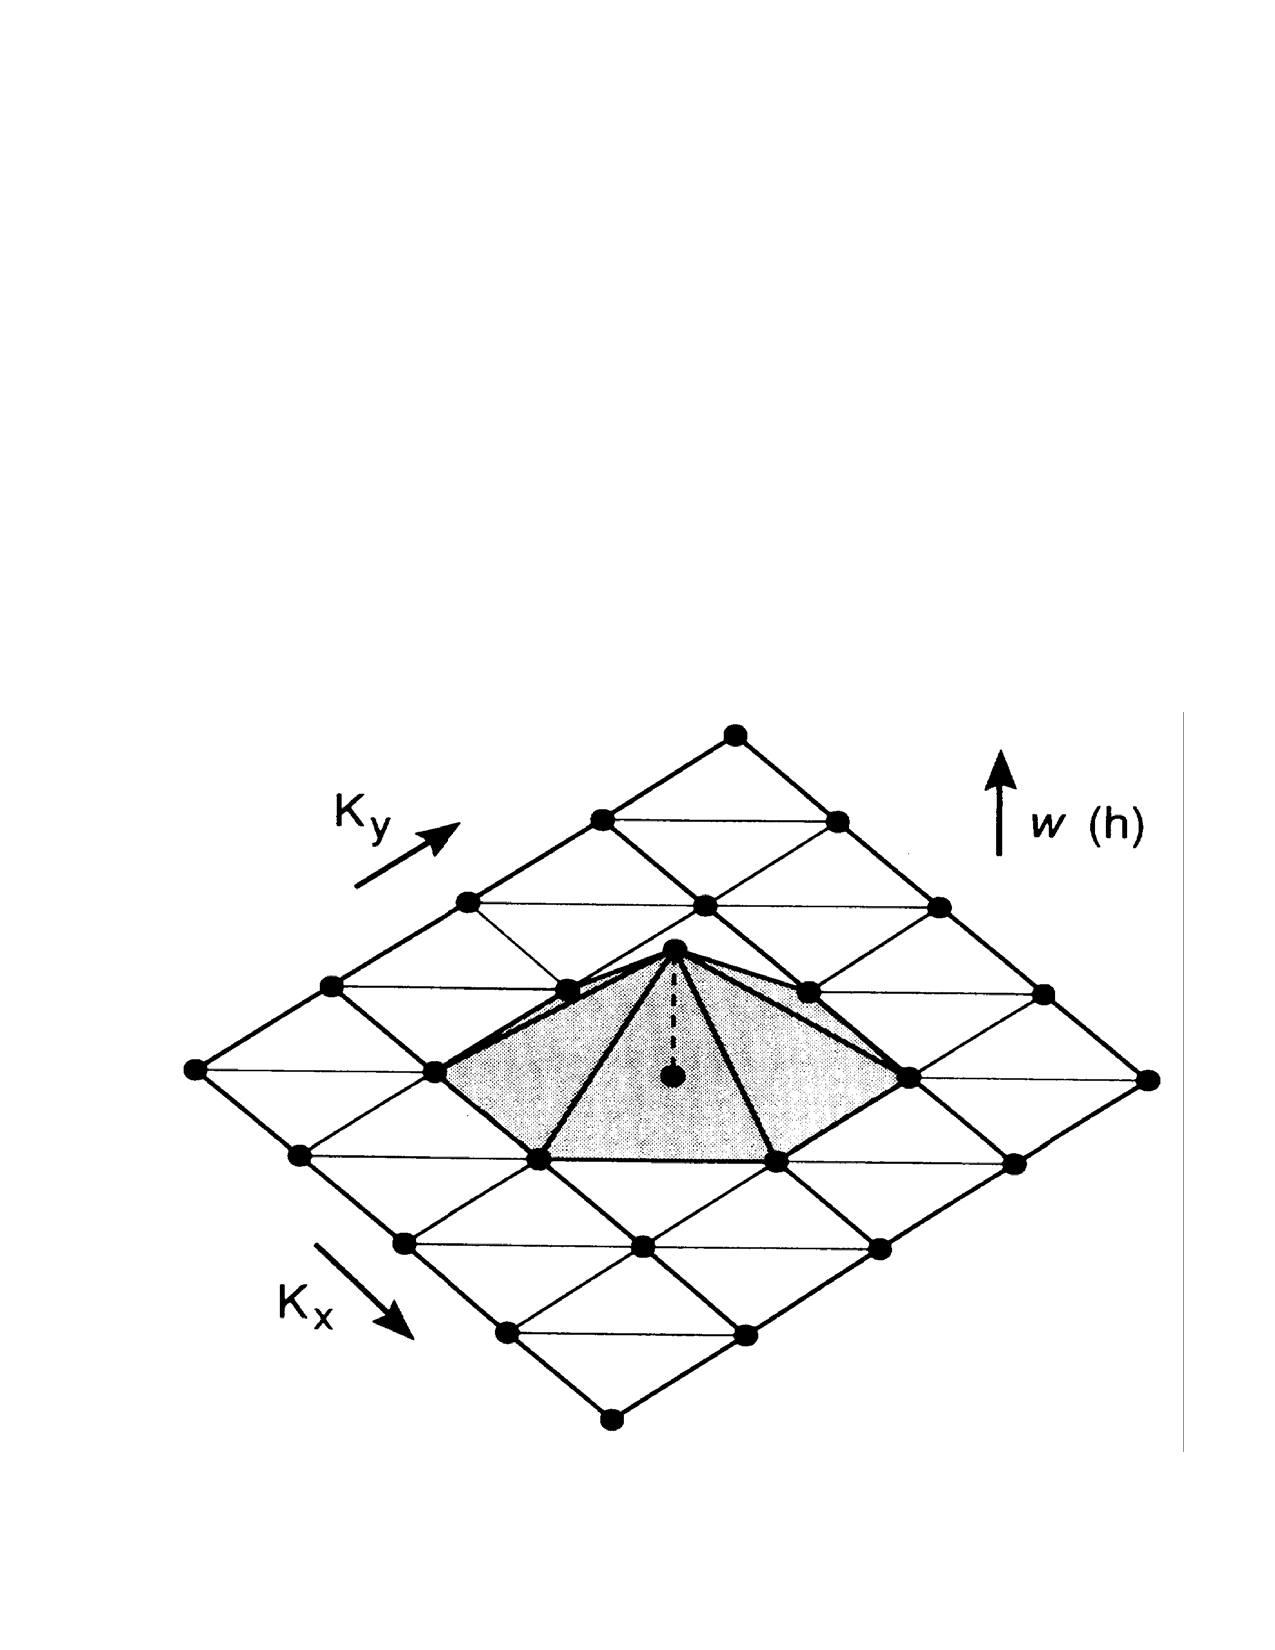
\includegraphics[height=1.75in,width=1.75in,viewport=0 30 565 505,clip]{Figures/dimen_Tetra.pdf}}
\end{figure}
}

\frame
{
	\frametitle{四面体布点方案}
	\begin{itemize}
	\item $\varepsilon_2<\varepsilon_F<\varepsilon_3$
		\begin{displaymath}
			\begin{aligned}
				\omega_1=&C_1+(C_1+C_2)\dfrac{\varepsilon_3-\varepsilon_F}{\varepsilon_{31}}+(C_1+C_2+C_3)\dfrac{\varepsilon_4-\varepsilon_F}{\varepsilon_{41}}\\
				\omega_2=&C_1+C_2+C_3+(C_2+C_3)\dfrac{\varepsilon_3-\varepsilon_F}{\varepsilon_{32}}+C_3\dfrac{\varepsilon_4-\varepsilon_F}{\varepsilon_{42}}\\
				\omega_3=&(C_1+C_2)\dfrac{\varepsilon_F-\varepsilon_1}{\varepsilon_{31}}+(C_2+C_3)\dfrac{\varepsilon_F-\varepsilon_2}{\varepsilon_{32}}\\
				\omega_4=&(C_1+C_2+C_3)\dfrac{\varepsilon_F-\varepsilon_1}{\varepsilon_{41}}+C_3\dfrac{\varepsilon_F-\varepsilon_2}{\varepsilon_{42}}
			\end{aligned}
		\end{displaymath}
		这里
		\vspace*{-10pt}
		\begin{displaymath}
			\begin{aligned}
				C_1&=\dfrac{V_T}{4V_G}\dfrac{(\varepsilon_F-\varepsilon_1)^2}{\varepsilon_{41}\varepsilon_{31}}\\
				C_2&=\dfrac{V_T}{4V_G}\dfrac{(\varepsilon_F-\varepsilon_1)(\varepsilon_F-\varepsilon_2)(\varepsilon_3-\varepsilon_F)}{\varepsilon_{41}\varepsilon_{32}\varepsilon_{31}}\\
				C_3&=\dfrac{V_T}{4V_G}\dfrac{(\varepsilon_F-\varepsilon_2)^2(\varepsilon_4-\varepsilon_F)}{\varepsilon_{42}\varepsilon_{32}\varepsilon_{41}}\\
			\end{aligned}
		\end{displaymath}
	\end{itemize}
}

\frame
{
	\frametitle{四面体布点方案}
	\begin{itemize}
	\item $\varepsilon_3<\varepsilon_F<\varepsilon_4$
		\begin{displaymath}
			\begin{aligned}
				\omega_1=&\dfrac{V_T}{4V_G}-C\dfrac{\varepsilon_4-\varepsilon_F}{\varepsilon_{41}}\\
				\omega_2=&\dfrac{V_T}{4V_G}-C\dfrac{\varepsilon_4-\varepsilon_F}{\varepsilon_{42}}\\
				\omega_3=&\dfrac{V_T}{4V_G}-C\dfrac{\varepsilon_4-\varepsilon_F}{\varepsilon_{43}}\\
				\omega_4=&\dfrac{V_T}{4V_G}-C\bigg[4-(\varepsilon_4-\varepsilon_F)\bigg(\dfrac1{\varepsilon_{41}}+\dfrac1{\varepsilon_{42}}\dfrac1{\varepsilon_{43}}\bigg)\bigg]
			\end{aligned}
		\end{displaymath}
		这里
		\begin{displaymath}
			C=\dfrac{V_T}{4V_G}\dfrac{(\varepsilon_4-\varepsilon_F)^3}{\varepsilon_{41}\varepsilon_{42}\varepsilon_{43}}
			\label{eq:weight-2-C}
		\end{displaymath}
	\item $\varepsilon_F>\varepsilon_1$
		\begin{displaymath}
			\omega_1=\omega_2=\omega_3=\omega_4=\dfrac{V_T}{4V_G}
		\end{displaymath}
	\end{itemize}
}

\frame
{
	\frametitle{四面体布点方案}
%类似地,可以有四面体方法态数目(\textrm{number of states})、态密度(\textrm{Density of States, DOS})$D_T(\varepsilon_i)$的贡献表达式,具体可参见文献\cite{PRB49-16223_1994}。
	为了减少统计四面体的数目,可以先找出第一\textrm{Brillouin-zone}的不可约部分。但这一策略有副作用,\textcolor{red}{由于不可约部分的不规则性,其中的四面体划分几乎不可避免地要人工干预,不利于编程求解}\\\textrm{Bl\"ochl}提出一个解决方法:\\
\begin{enumerate}
	\item 利用\textrm{Monkhorst-Pack}方案\upcite{PRB13-5188_1976}首先在第一\textrm{Brillouin-zone}内生成等体积的平行六面体网格。
	\item 依次给每个点编号:
\begin{displaymath}
	\boxed{N=1+\dfrac{i-i_0}2+(n_1+1)\left[\dfrac{j-j_0}2+(n_2+1)\dfrac{k-k_0}2\right]}
\end{displaymath}
其中$i,j,k$分别是该$\vec k$~点沿倒格矢$\mathbf{b}_i(i=1,2,3)$的序数的二倍,$i_0,j_0,k_0$是\textrm{Monkhorst-Pack}方法中点的偏移量,有偏移则为1,否则为0。
\end{enumerate}
}

\frame
{
	\frametitle{四面体布点方案}
\begin{enumerate}
	\setcounter{enumi}{2}
	\item 编号之后建立标识数组,其位置与该位置储存的元素值相同,例如,第一个位置存储“$1$”,第二个位置存储“$2$”,依次类推
	\item 然后从第一个位置开始,利用对称群的操作矩阵对每个点坐标作用,并与数组中其他点的坐标进行比较,如果彼此相同且后者的编号大于前者,即将后者的元素值改为前者\\\textcolor{blue}{对全部数组操作完毕,可以挑出所有不可约$\vec k$~点:\\只有当$\vec k_i$~为不可约$\vec k$~点时,其编号才与其存储位置相同}。
	\item 为了计算方便,可以对所有这些不可约$\vec k$~点按存储位置的顺序重新编号,即从“$1$”到“$\vec k_{\mathrm{irr}}(\max)$”。数组中的各个元素也相应的改为新的编号。这样整个第一\textrm{Brillouin-zone}中的点都可用不可约点标记。
\end{enumerate}
}

\frame
{
	\frametitle{四面体布点方案}
下一步讨论四面体的自动划分过程

以下八组坐标代表的点构成平行六面体:
\begin{displaymath}
	\begin{aligned}
		&(l,m,n)\rightarrow 1,&(l+1,m,n)\rightarrow 2\\
		&(l,m+1,n)\rightarrow 3,&(l+1,m+1,n)\rightarrow 4\\
		&(l,m,n+1)\rightarrow 5,&(l+1,m,n+1)\rightarrow 6\\
		&(l,m+1,n+1)\rightarrow 7,&(l+1,m+1,n+1)\rightarrow 8
	\end{aligned}
\end{displaymath}
为了尽量减小插值引起的误差,可以取此平行六面体中最短的体对角线作为等体积的六个四面体的公共对角线,设为$3-6$,则可以采用下面6组途径确定这六个四面体的各个顶点:
\begin{displaymath}
	\begin{aligned}
		1\rightarrow2\rightarrow3\rightarrow6\quad&1\rightarrow3\rightarrow5\rightarrow6\quad&2\rightarrow3\rightarrow4\rightarrow6\\
		3\rightarrow5\rightarrow6\rightarrow7\quad&3\rightarrow4\rightarrow6\rightarrow8\quad&3\rightarrow6\rightarrow7\rightarrow8
	\end{aligned}
\end{displaymath}
}

\frame
{
	\frametitle{四面体布点方案}
\begin{figure}[h!]
\centering
\vspace*{-0.28in}
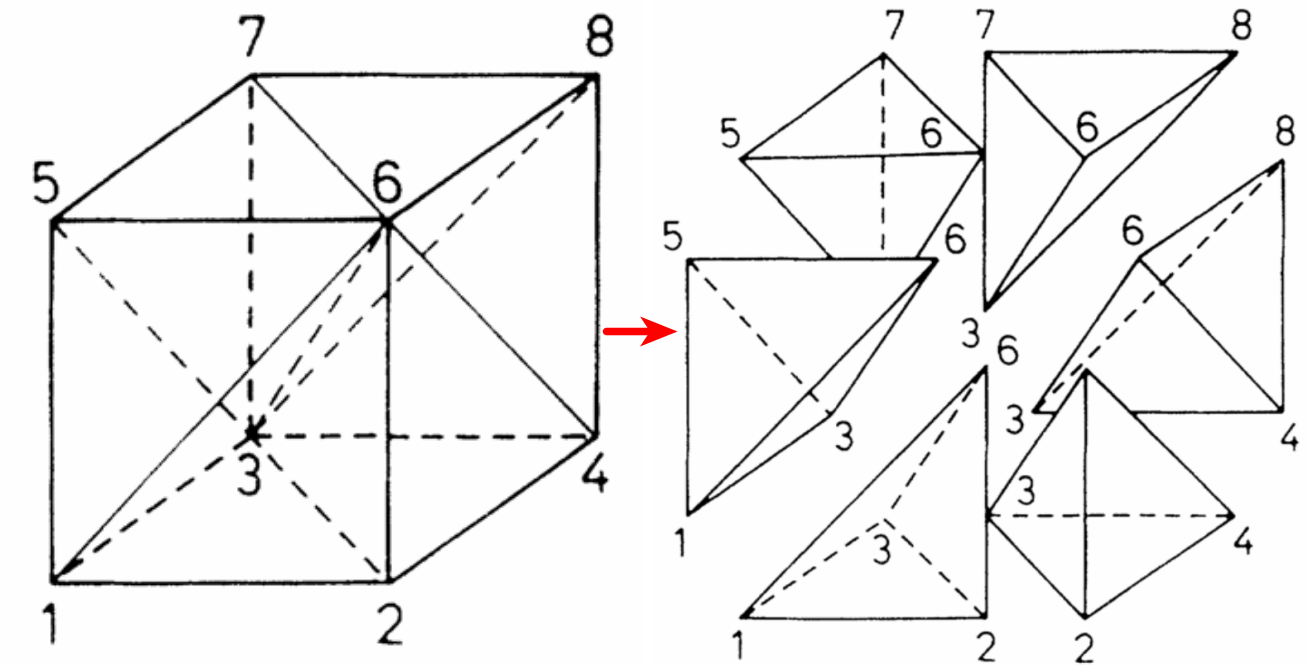
\includegraphics[height=1.25in,width=3.00in,viewport=0 0 1350 705,clip]{Figures/submesh_Tetra.png}
\caption{\small Breakup of a submesh cell into six tetrahedra.}%(与文献\cite{EPJB33-47_2003}图1对比)
\label{Fig:Submesh_Tetra}
\end{figure}
对每个平行六面体重复上述过程,将第一\textrm{Brillouin-zone}划分为体积相等的若干四面体,每个四面体的顶点可用标识数组中的不可约点标记。将这四个顶点的标号按升序排列,可以方便地确定等价四面体(简并度)\\
这个过程保证了\textcolor{red}{只用不可约点上的信息进行整个第一\textrm{Brillouin}区的积分,无须考虑如何划定其不可约部分}\\
%上述过程可以避免Kleinman所说的计算误差,而且整个过程可以通过程序自动实现而无须人工干预。
上述过程可以避免计算误差,而且整个过程可以通过程序自动实现而无须人工干预
}

%\frame
%{
%\begin{figure}[h!]
%\centering
%\vspace*{-0.25in}
%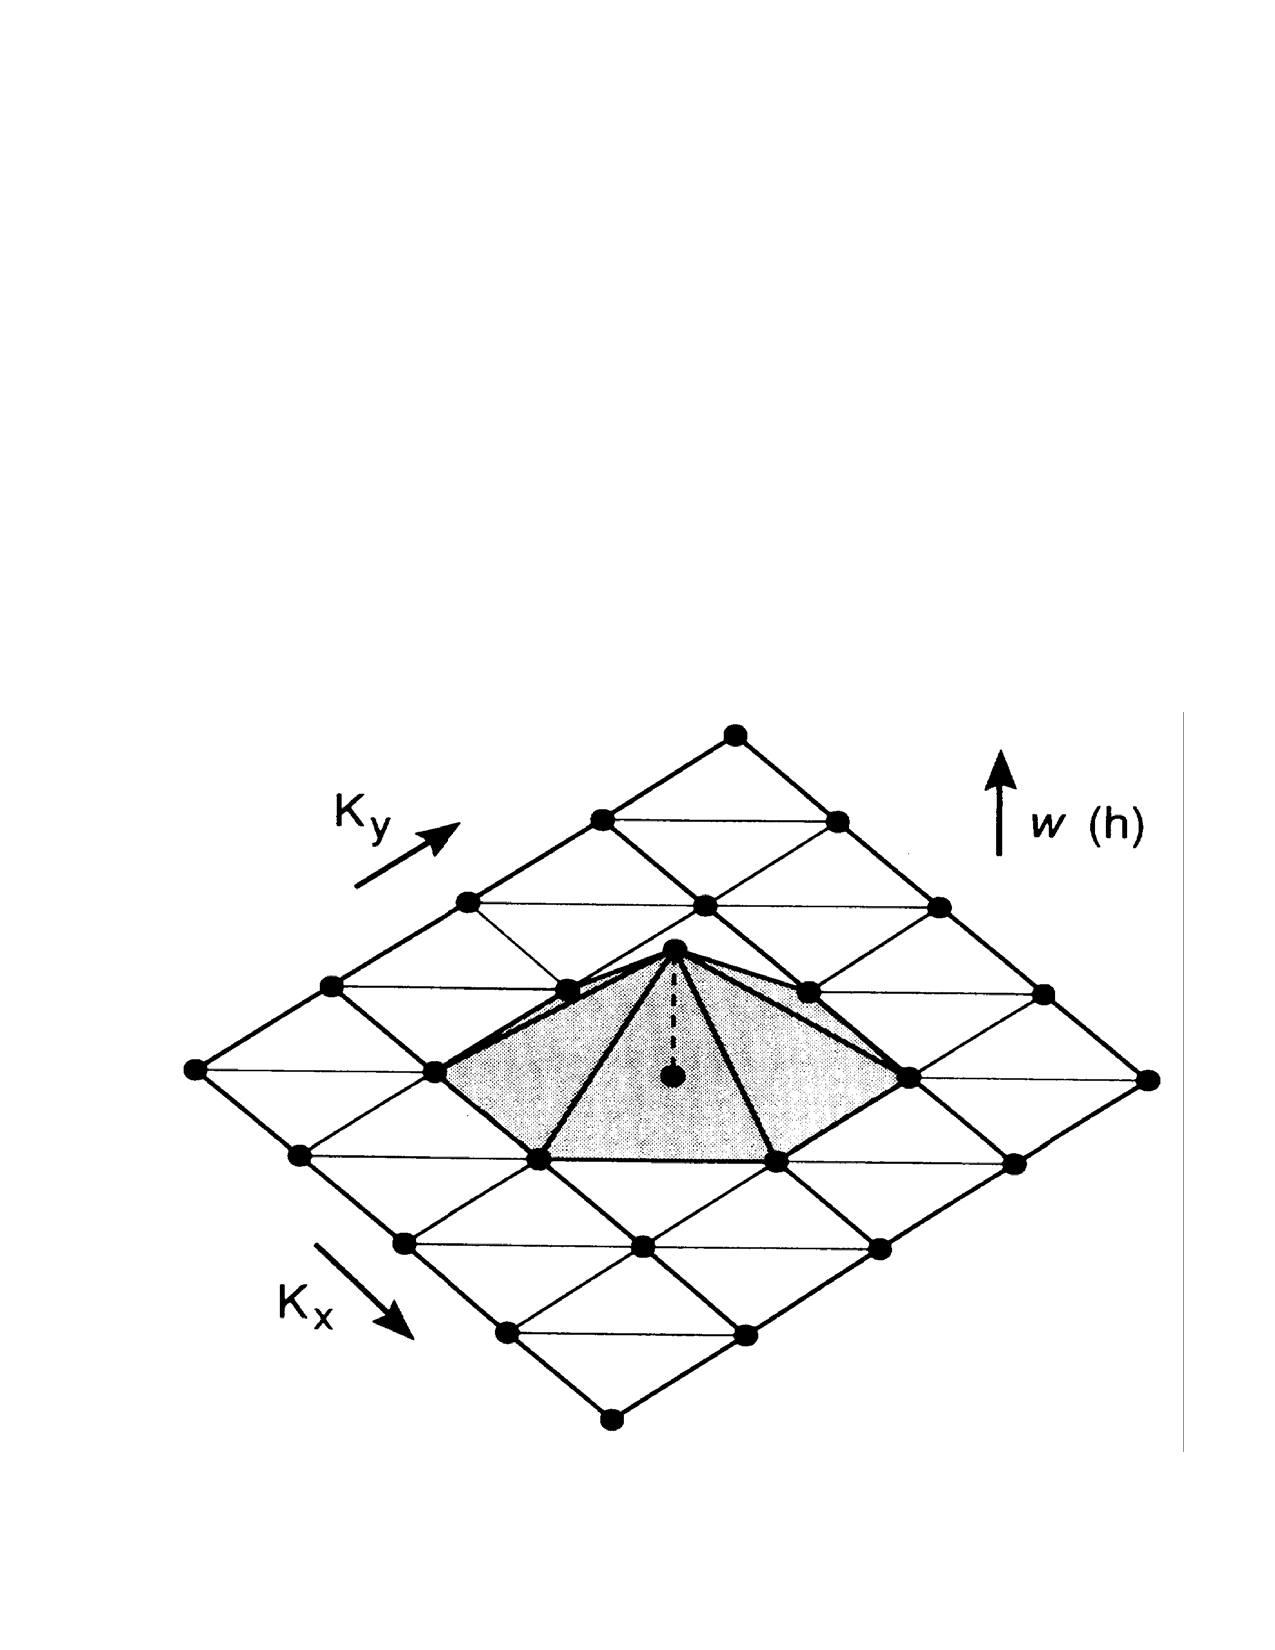
\includegraphics[height=2.75in,width=3.05in,viewport=0 30 565 505,clip]{Figures/dimen_Tetra.pdf}
%\caption{\small Two-dimensional schematic illustration of the function $w_j(\vec k)$.}%(与文献\cite{EPJB33-47_2003}图1对比)
%\label{Fig:Submesh_Tetra}
%\end{figure}
%}

\appendix
%------------------------------------------------------------------------Reference----------------------------------------------------------------------------------------------
%\begin{thebibliography}{99}
%-----------------------------------------------------------------------------------------------------------------------------------------------------------------------%
%\frame
%{
%\frametitle{主要参考文献}
%{\small
%\bibitem{Singh_Book}\textrm{D. J. Singh. \textit{Plane Wave, PseudoPotential and the LAPW method} (Kluwer Academic, Boston,USA, 1994)}					%
%  \nocite{*}																				%
%}
%}
%\end{thebibliography}

\begin{thebibliography}{99}
\frame
{
\frametitle{主要参考文献}
{\small
%	\bibitem{Huang_Han}黄昆\:原著、韩汝琦\:改编, {\textit{固体物理学}}\:高等教育出版社, 北京, 1988
%	\bibitem{Xie_Lu}谢希德、陆栋\:主编, {\textit{固体能带理论}}\:复旦大学出版社, 上海, 1998
	\bibitem{PRB49-16223_1994}\textrm{P. E. Bl\"ochl, O. Jepsen and O. K. Andersen \textit{Phys. Rev.} B, \textbf{49} (1994), 16223}
	\bibitem{PRB13-5188_1976}\textrm{H. J. Monkhorst and J. D. Pack \textit{Phys. Rev.} B, \textbf{13} (1976), 5188}
        \bibitem{Singh_Book}\textrm{D. J. Singh. \textit{Plane Wave, PseudoPotential and the LAPW method} (Kluwer Academic, Boston,USA, 1994)}
}
\nocite*{}
}
\end{thebibliography}
%{\small
%\phantomsection\addcontentsline{toc}{section}{Bibliography}	 %直接调用\addcontentsline命令可能导致超链指向不准确,一般需要在之前调用一次\phantomsection命令加以修正	%
%\bibliography{Myref}																			%
%\bibliographystyle{mybib}																		%
%  \nocite{*}																				%
%}
%-----------------------------------------------------------------------------------------------------------------------------------------------------------------------%


%-----------------------------------------------------------Beamer下不建议使用bib,因为涉及分页--------------------------------------------------------------------------%
%{\small
%\phantomsection\addcontentsline{toc}{section}{Bibliography}	 %直接调用\addcontentsline命令可能导致超链指向不准确,一般需要在之前调用一次\phantomsection命令加以修正	%
%\bibliography{Myref}																			%
%\bibliographystyle{mybib}																		%
%  \nocite{*}																				%
%}

%------------------------------------------------------------------------------------------------------------------------------------------------------------------------------%

%-------------------------------------------------------------------------Thanks------------------------------------------------------------------------------------------------
%\section{致谢}
%\frame
%{
%\frametitle{致$\quad$谢}
%\begin{itemize}
%    \setlength{\itemsep}{20pt}
%  \item 感谢本团队高兴誉、吴泉生、宋红州等各位老师参与的讨论
%  \item 感谢莫所长、宋主任以及软件中心各位老师和同事
%  \item 感谢王崇愚先生的帮助
%\end{itemize}
%}

\logo{}									%不显示logo
\frame
{
\vskip 60 pt
%\hskip 10pt \textcolor{blue}{\Huge 感谢答辩委员会各位老师\,\textrm{!}}\\
\vskip 35 pt
\hskip 60pt \textcolor{blue}{\Huge 谢谢大家\:!}
%\vskip 15 pt
%\hskip 40pt \textcolor{blue}{\Huge \textrm{for your attention\:!}}
}

%-------------------------------------------------------------------------------------------------------------------------------------------------------------------------------

\clearpage
%\end{CJK*}
\end{document}
